\documentclass[letterpaper]{article}
\usepackage[submission]{aaai2027}
%\usepackage{times}
%\usepackage{helvet}
%\usepackage{courier}
\usepackage[hyphens]{url}
\usepackage{graphicx}
\urlstyle{rm}
\def\UrlFont{\rm}
\usepackage{natbib}
\usepackage{caption}
\frenchspacing
\setlength{\pdfpagewidth}{8.5in}
\setlength{\pdfpageheight}{11in}
\usepackage{algorithm}
\usepackage{algorithmic}
\usepackage{booktabs}
\usepackage{amsmath}
\DeclareMathOperator*{\argmin}{arg\,min}
\DeclareMathOperator*{\argmax}{arg\,max}
\usepackage{multirow}
\usepackage{tikz}
\usetikzlibrary{arrows.meta,positioning,fit}
\pdfinfo{
/TemplateVersion (2027.1)
}

\setcounter{secnumdepth}{0}

\title{Use LLMs to Build Repair Tools, Not Patch Generation: \\ Cost-Effective Automated Program Repair}
\author{Anonymous submission}
\affiliations{}

\begin{document}
\maketitle

\begin{abstract}

Automated program repair can give every student in a programming course immediate feedback. Reference-guided repair transplants from the correct programs a class has already submitted and costs nothing per submission, but fails where the pool holds no structurally matching program. LLM-based repair has no such limit, yet it issues one query per submission, so spending grows with enrollment and recurs every term while the queries to one assignment re-read the same specification and re-derive the same few misconceptions hundreds of times. We present \textsc{CoEP}, in which the model writes the repair \emph{tool} rather than the patch. Once per assignment, a builder LLM turns worked pairs drawn from the class's own submissions into a module of misconception-named rewrite rules over a reference-guided transplant, validated against the instructor's test cases and then frozen. Submissions are repaired by that module with no model at all, and only what it abstains on, or what it patches more heavily than the program is long, takes a conventional call; the repairs it cannot make are distilled back into rules it keeps, so the artifact develops with the assignment it serves. What is deployed is not a model but code that can be read, audited, and that names the misconception behind every repair.
\end{abstract}

\section{Introduction}


Every year, thousands of students enroll in programming courses, and online judges accumulate millions of submissions to the same set of problems. With the rapid growth of Computer Science enrollment, providing personalized and timely feedback on programming assignments has become a significant challenge, requiring substantial time and effort from faculty \citep{yi2017feasibility,hu2020re}.


Automated Program Repair (APR) has emerged as a promising solution to this challenge, aiming to deliver automated and personalized feedback to students about their programming errors \citep{gulwani2018automated,sarfgen2018,hu2020re,ahmed2022verifix}. Reference-guided APR aligns a buggy program with a correct program for the same problem and transplants the differing region. It uses no model at deployment, so it runs offline and deterministically at no marginal cost per submission. Its applicability depends on the pool of correct programs containing a structurally matching correct program: when the alignment is not possible, the tool reports a structural mismatch and the program is returned unrepaired \citep{orvalho2025}.


More recently, Large Language Models (LLMs) trained on code have shown great potential in repairing programs \citep{xia2022less,xia2024automated,zhang2024pydex,liu2024fastfixer,yang2024cref}. LLM-based APR does not require a matching reference, so it applies where a structural mismatch would otherwise arise, and it extends beyond introductory exercises to harder problems. What concerns us is how it is deployed. The default is one model query per buggy program, so spending, latency, and dependence on an external service all scale with the number of submissions and recur every term. Queries to the same assignment also share most of their content: hundreds of students attempt one problem and their failures cluster into a few recurring misconceptions \citep{gulwani2018automated,hu2020re}, so the model re-reads one specification and re-derives one mistake many times over. Cheaper tiers and prompt caching lower the price of a call \citep{anthropiccaching,openaicaching} but leave the number of calls unchanged.

\begin{figure}[t]
\centering
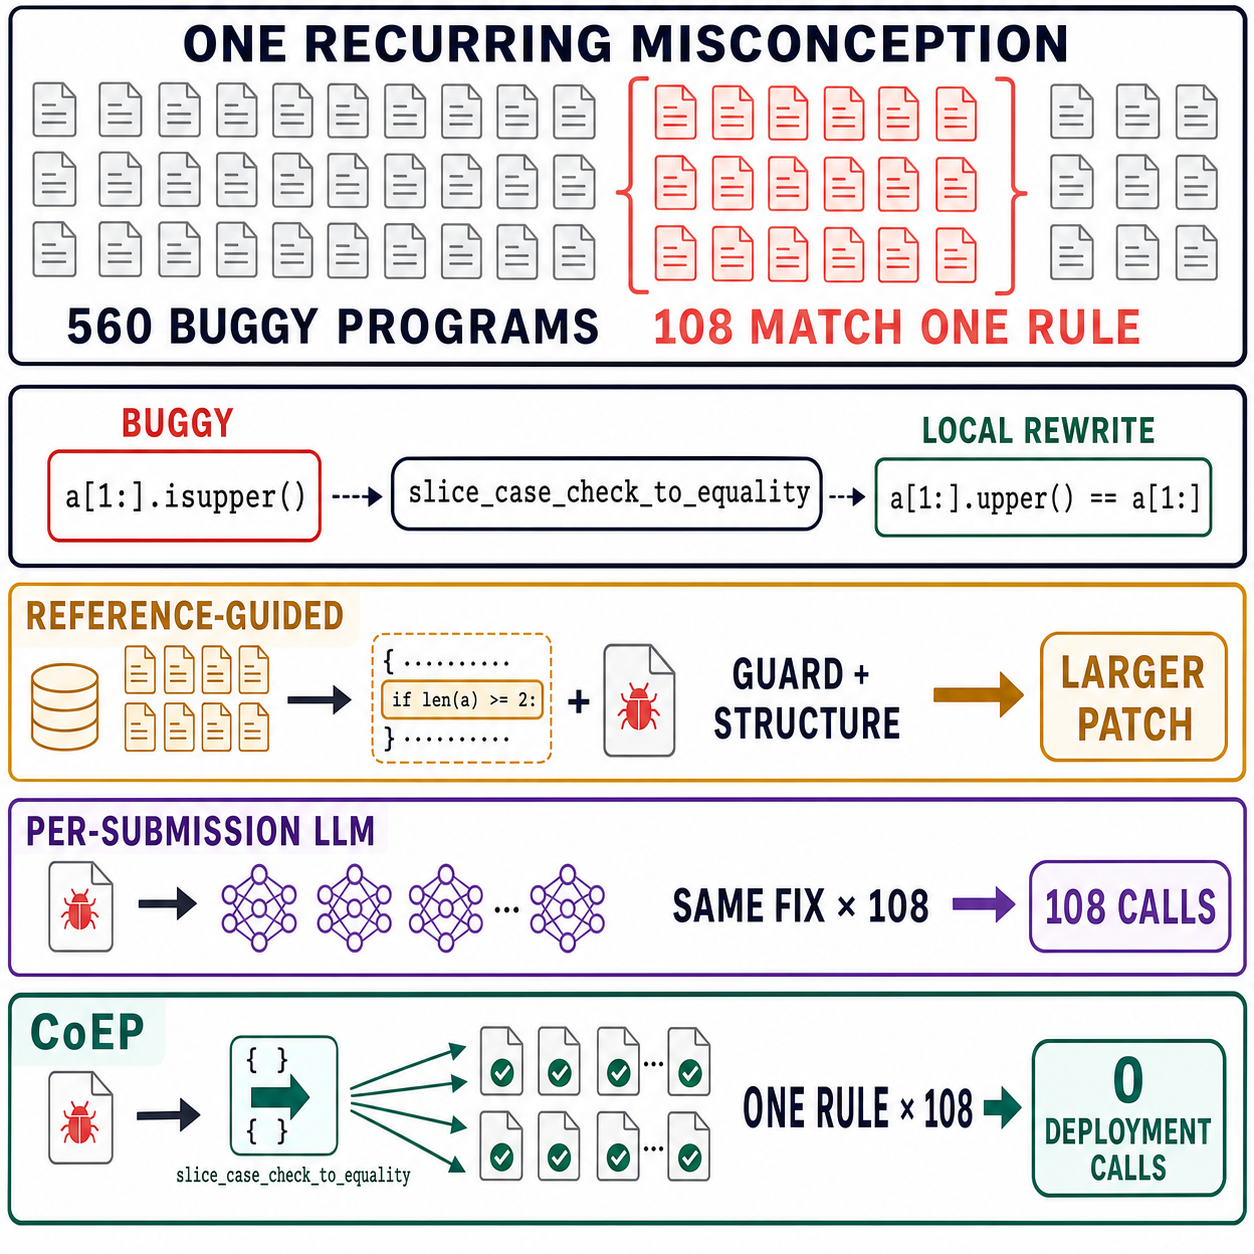
\includegraphics[width=0.86\columnwidth]{figures/fig_example_recurring_bug_comparison_gpt2.png}
\caption{Example of \textsc{CoEP}: A recurring misconception on cAPS lOCK and
 the rule that repairs it.}
\label{fig:example}
\end{figure}


In this paper, we propose \textsc{CoEP} (\underline{Co}st-\underline{E}ffective \underline{P}rogram repair), in which the model writes the repair \emph{tool} rather than the patch generation. The model is invoked once per problem instead of once per submission, and the product of that invocation is not a single repair but an executable program that handles every submission to the problem. An LLM agent receives the problem description, its test cases, and a clustered sample of (buggy, fixed) program pairs drawn from the class, and authors AST rewrite rules named after the misconceptions they repair. These rules run atop a shared symbolic substrate of a generic edit library and reference-guided minimal-hunk transplant from the pool of correct programs. Figure~\ref{fig:example} shows one such rule. On cAPS lOCK, 108 of 560 buggy programs test a word's tail with \texttt{a[1:].isupper()}, which is \texttt{False} on the empty tail of an input like \texttt{"Z"}. Repairing them one at a time re-derives the same fix 108 times, and a transplant must bring in a length guard with the structure around it. One rule instead rewrites that test in place, repairs all 108, of which the builder was shown 64 and never saw the other 44, at no deployment cost. Every candidate is validated against the instructor's test cases before it is kept, so the tool cannot self-report success and a defective one abstains rather than answers wrongly. Only what it abstains on, and what it patches more heavily than the program is long, escalates to a conventional call, so coverage is never sacrificed. Model spend therefore moves from a marginal cost that scales with submissions to a fixed one that scales with problems, and what a student's submission meets is code that can be read and audited, running offline inside the institution.


Our experiments with 2{,}970 buggy programs across 11 problems from a CS1 corpus and an online judge reveal that the synthesized tool outperforms Refactory, the strongest reference-guided repairer that runs on our data, on its own corpus and metric, repairing more programs with smaller patches. Against per-submission LLM repair it matches coverage while modifying less of the student's program, for a fraction of the model spend, and it recovers its one-off build cost within tens of submissions per problem. An ablation separates the layers. Where assignments already carry hundreds of correct submissions the reach is the substrate's and the rules add smaller patches and a misconception label; restrict the pool and the balance inverts, the substrate repairing 8.9\% of held-out submissions where the same tool with its rules repairs 29.5\%. Those two are what a per-submission call cannot amortize, since a call yields a patch but leaves no reusable artifact behind.


In summary, this paper makes the following contributions:
\begin{itemize}
  \item We reformulate APR for programming assignments so that the model authors a repair tool once per assignment rather than a patch per submission, leaving no model in the deployed system;
  \item We present \textsc{CoEP}, which synthesizes misconception-named rewrite rules atop a reference-guided transplant, and keeps developing the tool by distilling the repairs it could not make into new rules;
  \item Experiments on real student submissions show that \textsc{CoEP} repairs more programs with smaller patches than a reference-guided tool, and matches per-submission LLM repair at an order of magnitude lower cost.
\end{itemize}

\section{Related Work}
\label{sec:related}


\textbf{APR for programming assignments.} Early work reuses the correct programs a class has already submitted. CLARA and Sarfgen align a buggy program with its structurally nearest correct program and transplant the differing blocks \citep{gulwani2018automated,sarfgen2018}, Verifix backs that alignment with formal verification \citep{ahmed2022verifix}, and Refactory widens the range of alignable programs by refactoring the pool to match the buggy program's structure \citep{hu2020re}. A second line learns the repair function from data: sequence models \citep{deepfix2017}, reinforcement learning over edits \citep{rlassist2019}, and PROSE-based induction of per-assignment transformations \citep{refazer2017}. Most recently, LLMs trained on code address the problem directly: PyDex targets student programs and prepends similar correct programs retrieved by test-case behaviour as few-shot examples \citep{zhang2024pydex}, ChatRepair adds multi-turn conversation \citep{xia2024automated}, CREF places a tutor in the loop \citep{yang2024cref}, FastFixer fine-tunes for faster per-query inference \citep{liu2024fastfixer}, and recent work extends to counterexample-guided minimal repair \citep{orvalho2025} and learner-tailored retrieval \citep{lsgen2026}. Alongside repair itself, OverCode clusters a class's programs to show an instructor which mistakes recurred \citep{overcode2015}, the same instructor-facing view our rule provenance yields as a by-product of repairing. % [번역] 모델이 도구를 만들게 하기. 이 논문이 수리에 적용한 재정식화는 다른 곳에서 이미 이루어졌다. Cai 등은 유능한 모델이 재사용 가능한 유틸리티를 한 번 작성하게 하고 값싼 모델이 그것을 여러 번 호출하게 해 비싼 모델을 과제 계열에 상각한다. Voyager는 경험에서 기술 라이브러리를 축적하고, TroVE와 ReGAL은 프로그램 과제에서 재사용 가능한 함수를 귀납하며, FunSearch는 점수 함수에 대해 프로그램을 진화시킨다. 수리가 이 계열에 더하는 것은 오라클이다. 추론 과제를 위해 유도된 도구는 그럴듯해 보이기 때문에 신뢰받는 반면, 우리가 내놓는 모든 패치는 학생이 보기 전에 교수자의 테스트 케이스로 실행되므로 결함 있는 규칙은 틀린 답이 아니라 기권으로 퇴화하고 도구는 모델 없이 배포될 수 있다. 부산물도 다르다. 각 규칙이 이름 붙은 오개념을 위해 작성되므로 학급을 수리하는 일이 곧 학급에 라벨을 다는 일이 된다.
\textbf{Letting a model build the tool.} The reformulation this paper applies to repair has been made elsewhere: a capable model writes a reusable utility once and cheaper calls reuse it \citep{toolmakers2024}, skills accumulate from experience \citep{voyager2024}, and functions are induced from programmatic tasks or evolved against a score \citep{trove2024,regal2024,funsearch2024}. What repair contributes is an oracle. A tool induced for reasoning is trusted because it looks right, whereas every patch ours emits is executed against the instructor's test cases first, so a defective rule degrades into abstention rather than into a wrong answer and the tool ships with no model behind it.

Three of these are close enough that their absence from our baselines needs stating. Refazer is the closest in spirit, since it also induces assignment-specific transformations, but it learns them from a student's own (before, after) edit, which neither corpus records. Verifix and the counterexample-guided repair of \citet{orvalho2025} both operate on C, through MaxSMT over C types and a C-specific MaxSAT fault localizer, while our corpora are Python. We therefore take Refactory and PyDex as the reference-guided and per-submission LLM lines. Existing approaches, reference-guided and LLM-based alike, either fix the repair procedure by hand in advance or re-derive it from the model on every submission; neither leaves behind a reusable artifact for the assignment. To remedy this gap, we have the model author that artifact once per assignment, and repair every later submission with it and no model at all.

\section{Approach}
\label{sec:approach}

\subsection{Task Definition}

A programming assignment provides a problem description $d$, a set of test cases $T = \{t_1, \dots, t_n\}$, and a set of submissions. Writing $p \models T$ when a program $p$ passes every test case in $T$, the submissions divide into the buggy programs $B = \{p : p \not\models T\}$ and the correct programs $R = \{p : p \models T\}$. Since the correct program used to repair a buggy program is a reference program, $R$ is also the pool of reference programs. Repairing the buggy programs produces a set of fixed programs $F$, with individual members denoted $b$, $r$, and $f$. To repair $b$ is to produce an $f$ with $f \models T$, and nothing weaker counts: an $f$ passing only some test cases is not a repair.

\begin{figure}[h]
  \centering
  \resizebox{\columnwidth}{!}{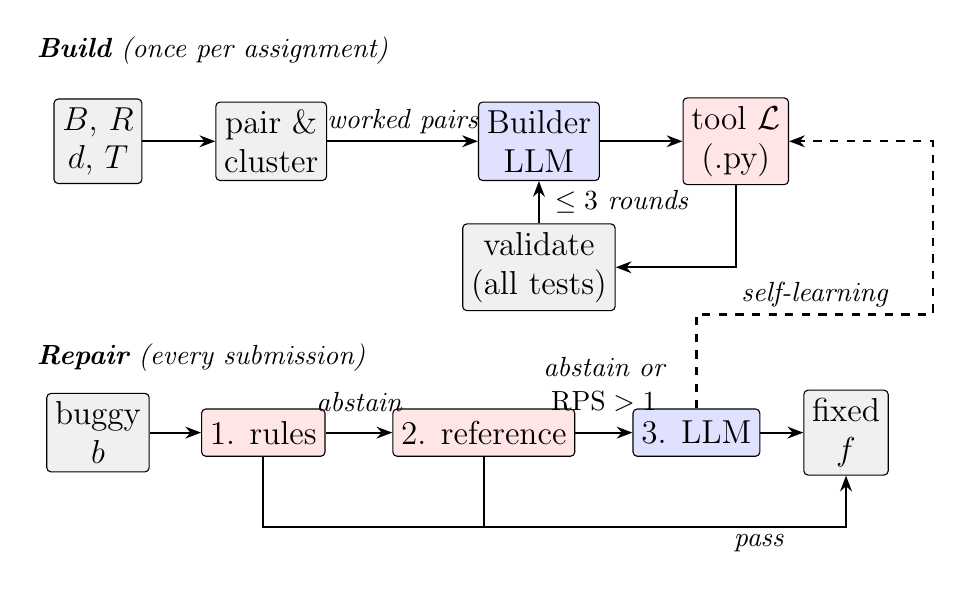
\begin{tikzpicture}[
    font=\large,
    box/.style={draw, rounded corners=1.5pt, align=center, inner sep=3pt, minimum height=6mm},
    llm/.style={box, fill=blue!12},
    loc/.style={box, fill=red!10},
    dat/.style={box, fill=black!6},
    arr/.style={-{Stealth[length=2mm]}, thick},
    lbl/.style={font=\normalsize\itshape, align=center}
  ]
  \node[lbl, anchor=west] at (-0.9, 1.15) {\textbf{Build} (once per assignment)};
  \node[dat] (spec) at (0, 0) {$B$, $R$\\$d$, $T$};
  \node[dat] (sel) at (2.2, 0) {pair \&\\cluster};
  \node[llm] (builder) at (5.6, 0) {Builder\\LLM};
  \node[loc] (tool) at (8.1, 0) {tool $\mathcal{L}$\\(.py)};
  \node[dat] (val) at (5.6, -1.6) {validate\\(all tests)};
  \draw[arr] (spec) -- (sel);
  \draw[arr] (sel) -- node[lbl, above=-1pt]{worked pairs} (builder);
  \draw[arr] (builder) -- (tool);
  \draw[arr] (tool.south) |- (val.east);
  \draw[arr] (val.north) -- node[lbl, right=2pt]{$\le 3$ rounds} (builder.south);
  \node[lbl, anchor=west] at (-0.9, -2.75) {\textbf{Repair} (every submission)};
  \node[dat] (sub) at (0, -3.7) {buggy\\$b$};
  \node[loc] (r1) at (2.1, -3.7) {1. rules};
  \node[loc] (r2) at (4.9, -3.7) {2. reference};
  \node[llm] (r3) at (7.6, -3.7) {3. LLM};
  \node[dat] (out) at (9.5, -3.7) {fixed\\$f$};
  \draw[arr] (sub) -- (r1);
  \draw[arr] (r1) -- node[lbl, above=4pt]{abstain} (r2);
  \draw[arr] (r2) -- node[lbl, above=4pt]{abstain or\\$\mathrm{RPS} > 1$} (r3);
  \draw[arr] (r3) -- (out);
  \draw[arr] (r1.south) -- (2.1, -4.9) -- node[lbl, below=-1pt, pos=0.85]{pass} (9.5, -4.9) -- (out.south);
  \draw[thick] (r2.south) -- (4.9, -4.9);
  \draw[arr, dashed] (r3.north) -- (7.6, -2.2) -- node[lbl, above=-1pt]{self-learning} (10.6, -2.2) -- (10.6, 0) -- (tool.east);
  \end{tikzpicture}}
  \caption{Overview of \textsc{CoEP}. LLM effort (blue) is spent once per assignment to build a local repair tool (red); at repair time the tool tries rules and a reference transplant first, so most submissions never reach a model. The dashed path is self-learning (\textsc{CoEP}\textsubscript{L+SL}).}
  \label{fig:arch}
\end{figure}

\subsection{Overview}


\textsc{CoEP} separates the two things a repair system does (Figure~\ref{fig:arch}). The \emph{build} happens once per assignment. A local step that costs no model call turns the class's own submissions into a small set of worked pairs, and a builder LLM turns those, together with $d$ and $T$, into a \emph{local repair tool} $\mathcal{L}$: an ordinary Python module with no model access. \emph{Repair} happens on every submission and consults $\mathcal{L}$ first. Given a buggy program $b$, the tool tries three strategies in increasing order of cost: its own rewrite rules, a transplant from a reference program, and, only if both abstain or the local patch is larger than the program it repairs, a single conventional model call. Whichever strategy first produces a candidate that passes every test case in $T$ supplies the fixed program $f$, so a model is involved in the third alone.


Three configurations follow from where we stop. \textsc{CoEP}\textsubscript{L} uses the tool alone and spends nothing per submission beyond CPU time. \textsc{CoEP}\textsubscript{LF} adds the model call for the submissions the tool cannot serve. \textsc{CoEP}\textsubscript{L+SL} adds self-learning: whenever the fallback repairs a submission the tool missed, the model generalizes that repair into a new named rule and the tool absorbs it, so an assignment's tool improves over a semester rather than staying frozen at whatever one build session produced.

\subsection{Build: Local Repair Tool}


\textbf{Worked pairs.} This step is local and costs no model call: the builder sees a \emph{chosen} sample of $B$ rather than all of it, one program per cluster, which on our assignments is 43--71\% of the pool. Let $\sigma(p)$ collect the node types of $p$'s AST read in breadth-first order, one sequence $\sigma_i(p)$ per top-level statement, and, with $\mathrm{lev}$ the Levenshtein distance between two such sequences, let $\delta(b,r)$ be the cost of the cheapest one-to-one matching $M$ of $b$'s sequences to $r$'s, $\min_{M} [\sum_{(i,j) \in M} \mathrm{lev}(\sigma_i(b), \sigma_j(r)) + \sum_{i \notin M} |\sigma_i(b)| + \sum_{j \notin M} |\sigma_j(r)|]$, so a missing or surplus definition costs what it is. Every buggy program takes as partner the reference program it is fewest edits from, $\pi(b) = \argmin_{r \in R} \delta(b, r)$, rather than the one that merely looks closest, and $\varepsilon(b)$ is the multiset of edit operations taking $b$ to $\pi(b)$, refined to a value-level alignment when the node-type one comes out empty, since a wrong identifier or literal is invisible to node types alone.


We then partition $B = C_1 \uplus \dots \uplus C_k$ by average linkage over cosine distance between TF-IDF vectors of the $\varepsilon(b)$, with $k$ chosen to maximize mean silhouette. Both choices were measured rather than assumed: a rule induced from a representative pays off on the members needing the \emph{same edit}, so grouping by shape fills the largest clusters with programs that merely look alike, and a fixed cut height is no smaller an assumption than a fixed $k$, one constant giving six-fold different granularity across our assignments. Each cluster contributes its \emph{modal} repair, $b^{\star}_i = \argmax_{b \in C_i} |\{b' \in C_i : \varepsilon(b') = \varepsilon(b)\}|$, degenerating to the medoid where no edit repeats. The medoid is the most typical \emph{program} and usually a multi-issue tangle; the smallest edit is the submission that came closest to correct, an outlier rather than a spokesman. The build set is $S = \{(b^{\star}_i, \pi(b^{\star}_i))\}_{i=1}^{k}$, ordered by increasing $\delta$, so a weak builder is shown each buggy program \emph{with} a reference program that repairs it and need only generalize the transformation.


\textbf{Rule authoring.} The builder LLM turns $(d, T, S)$, with $T$ shown as up to eight example cases, into the assignment-specific tool $\mathcal{L}_0$: a module of AST rewrite rules, each named after the misconception it targets and tagged with the failure symptoms it addresses. A rule is a \emph{candidate generator}, a map $\rho$ from a program to a set of candidates, under a strict contract: it splices its edit as a source-span replacement rather than re-rendering the module, it proposes rather than claims, and it never rewrites a whole function. A rule that cannot express a targeted edit, that raises, or that runs past a two-second alarm yields $\rho(p) = \emptyset$ and the submission escalates.


\textbf{Generate--validate--refine.} A single-shot module can contain its own defects, so the harness closes the loop on the build set, refining from execution feedback \citep{selfrefine2023,reflexion2023}. Write $\mathrm{cov}(\mathcal{L})$ for the fraction of $S$ whose buggy half the rule search below repairs, $|\{(b, \cdot) \in S : \exists\, c \in \mathcal{L}^{*}(b),\, c \models T\}| / |S|$, with $\mathcal{L}^{*}(b)$ the candidate set that search enumerates; the transplant sits deliberately outside it, so a round is scored on the rules the builder wrote and not on the substrate underneath them. Coverage is measured by \emph{executing} $T$, never from the module's own claim. While $\mathrm{cov}(\mathcal{L}_j) < 1$ the harness returns the still-failing sources for revision, giving $\mathcal{L}_{j+1}$, for up to $r_{\max}{=}3$ builder calls; the frozen tool is $\mathcal{L} = \argmax_{j \le r_{\max}} \mathrm{cov}(\mathcal{L}_j)$, ties going to the earliest round. Build cost is exactly the token count of these exchanges, measured from the raw strings.

\subsection{Repair: Rules, Reference, LLM}


Given $b$, the frozen tool $\mathcal{L}$ tries three strategies in increasing order of cost and returns the first candidate $c$ it can verify with $c \models T$. The first two use no model; only the third spends a call.


\textbf{Rule-based repair.} The rules are composed by a symptom-ordered search over layers: $\Lambda_0 = \{b\}$ and $\Lambda_{j+1} = (\bigcup_{p \in \Lambda_j} \bigcup_{\rho \in \mathcal{L}} \rho(p)) \setminus \bigcup_{i \le j} \Lambda_i$, with $b$'s failing-test signature ordering the $\rho$ whose declared symptoms match. Every candidate in $\Lambda_{j+1}$ is validated before $\Lambda_{j+2}$ is enumerated, so the returned repair is by construction the shallowest $c$ with $c \models T$, and $\mathcal{L}^{*}(b) = \bigcup_j \Lambda_j$. A handful of always-on rules for the slips every class makes, comparison flips and off-by-one range and index shifts, sit alongside whatever the builder writes; they invert the classical mutation-operator space \citep{mutants2014,par2013,tbar2019}. Every surviving patch carries the ordered rule names behind it, provenance that aggregates into a per-class \emph{misconception profile}.


\textbf{Reference-based repair.} Most student bugs need a structural edit no rule expresses; $R$ supplies it. Let $H(b, r)$ be the differing line-hunks between $b$ and one of the eight structurally nearest reference programs $r$, taken both raw and with $r$'s variables renamed to the student's, parameters by position and locals by first binding, and let $b \oplus h$ be $b$ with the hunks $h \subseteq H(b,r)$ applied. We validate the 300 smallest $h$ with $1 \le |h| \le 3$ in increasing order of lines changed and return $\argmin_{h} \mathrm{RPS}(b, b \oplus h)$ over the first five satisfying $b \oplus h \models T$, abstaining when none does, so the exact tree-edit score, the distance from $b$ to $b \oplus h$ normalized by the size of $b$ and defined with the other metrics in the Experimental Setup, is paid only on the handful that pass. This is reference reuse in the lineage of CLARA, Sarfgen, and Refactory \citep{gulwani2018automated,sarfgen2018,hu2020re}, at hunk granularity rather than the block granularity those systems use.


\textbf{LLM-based repair.} Conventional LLM-based APR maps every buggy program to a query $\mathrm{LLM}(d, T, b)$. \textsc{CoEP} keeps that call for the submissions the local strategies cannot serve, and its cost is counted against \textsc{CoEP} in every comparison. Writing $f_{\mathrm{loc}}$ for the local result, it fires when $f_{\mathrm{loc}} = \mathrm{fail}$ or $\mathrm{RPS}(b, f_{\mathrm{loc}}) > 1$. Abstention is not the only trigger because the acceptance test is the instructor's suite, which says nothing about patch size: the transplant can return a $c \models T$ larger than the student's whole program, while the rule layer must return $\emptyset$ whenever it cannot express a targeted edit. The threshold gives the transplant the same contract, since a patch larger than the program it repairs is a rewrite, not a repair, under any assignment's standards. The call is strengthened to match the student's strategy by attaching the minimum-edit reference program $r = \pi(b)$, the same pairing the build uses, and we keep $\argmin_{f \in \{f_{\mathrm{loc}},\, \mathrm{LLM}(d,T,b,r)\},\ f \models T} \mathrm{RPS}(b, f)$, abstaining when neither passes, so escalating can cost a call but never coverage or patch size.


The threshold is a constant rather than a quantity calibrated per assignment. We chose it that way because its value is a definition and not a fitted number. Across the 29 settings we measured the repair rate is identical to four decimals and spend stays within \$12.47--\$15.61, so the choice carries no conclusion; the supplement plots them.


\textbf{Self-learning.} From an escalated pair $(b, f)$ the LLM writes a new named rule $\rho'$, kept only if $\exists\, c \in (\mathcal{L} \cup \{\rho'\})^{*}(b)$ with $c \models T$, in which case $\mathcal{L} \leftarrow \mathcal{L} \cup \{\rho'\}$. Absorption writes to a staging copy the evaluated pass never consults, so no submission's outcome depends on which preceded it, and the accumulated rules are a separate artifact, evaluated by a second frozen pass and priced to themselves. This is the \textsc{CoEP}\textsubscript{L+SL} configuration; it spends calls only on submissions that already escalated, so it too leaves the build claim untouched.


The first two strategies run on a CPU in ${\sim}2$--$3$\,s per submission and offline. Under \textsc{CoEP}\textsubscript{L} no student code leaves the institution once the tool is built, though the build sends the worked pairs and \textsc{CoEP}\textsubscript{LF} sends each escalated submission: the guarantee belongs to the configuration, not the method. Rule application and transplant are themselves deterministic; the enumeration that feeds them is bounded by a wall clock, so under heavy load fewer candidates are examined and the tool may abstain where it would otherwise repair. A defective tool fails, never returning a wrong repair, because the harness re-validates every patch before a student sees it.

\section{Experiments}

\subsubsection{Research Questions.}


\begin{itemize}
  \item \textbf{RQ1}: What is the cost impact of synthesizing a repair tool once per assignment, compared to querying an LLM once per submission?
  \item \textbf{RQ2}: How effective is \textsc{CoEP} in repairing programming assignments compared to state-of-the-art reference-guided and LLM-based repair approaches?
  \item \textbf{RQ3}: How does the LLM-authored rule layer impact the performance of \textsc{CoEP}?
  \item \textbf{RQ4}: How helpful is it to absorb the repairs of escalated submissions back into the tool as new rules?
\end{itemize}

\subsubsection{Baselines.}
\label{sec:setup}

We compare \textsc{CoEP} against the two mainstream lines of program repair for programming assignments: (1) \textbf{Refactory} \citep{hu2020re}, which refactors the class's correct programs to match each buggy program's structure and transplants the divergent blocks;  (2) \textbf{PyDex} \citep{zhang2024pydex}, which sends each buggy program to the model in its few-shot layout with the three most similar (buggy, correct) exemplars retrieved from the class pool, samples $K{=}10$ candidates per submission, filters them by the test oracle, and returns the survivor closest to the student's program. We issue the ten as separate requests and bill all ten, where the original draws them from one; billing the prompt once would put PyDex at \$231 and the factor at 17 rather than 21.6. (3) \textbf{PyDex\textsubscript{PC}} re-prices the same queries under \emph{prompt caching}. Providers let a query reuse the key--value tensors computed for an identical leading prefix of an earlier one, so the cached prefix is billed at roughly a tenth of the input rate and need not be re-encoded \citep{anthropiccaching,openaicaching}. \textsc{CoEP} itself is evaluated in three configurations. \textbf{\textsc{CoEP}\textsubscript{L}} runs the frozen local tool alone with no deployment LLM use, accepting any patch the test oracle passes, which is the acceptance rule Refactory uses. \textbf{\textsc{CoEP}\textsubscript{LF}} adds the per-submission fallback on abstentions and on passing local patches above $\mathrm{RPS}=1$. \textbf{\textsc{CoEP}\textsubscript{fw}} is the framework alone, the same tool with the builder's rules removed and the always-on rules and the transplant left in place, which calls no model at any point. \textbf{\textsc{CoEP}\textsubscript{L+SL}} re-runs \textsc{CoEP}\textsubscript{L} with the self-learned rules merged and frozen beforehand, so the arm is order-independent; its induction calls are priced to it.



\subsubsection{Datasets.}

We evaluate on 11 problems and 2{,}970 buggy programs drawn from two real-student corpora: five CS1 assignments contributing 1{,}783 buggy and 2{,}442 correct programs at 7.4 test cases per assignment, and six Codeforces problems contributing 1{,}187 buggy and 698 correct at 35.5 test cases. The first five are a first-year university course's assignments with every submission its students wrote, released with Refactory \citep{hu2020re} and since standard in this literature \citep{zhang2024pydex}. The other six come from Codeforces, whose submissions the open-r1 release mirrors \citep{penedo2025codeforces}, sampled at ratings 800 through 2000 across five official bands \citep{cfratings} and restricted to problems whose complete official test suites are public, so the oracle is the judge's own. Every submission a corpus labels buggy is a repair target for every arm, so the denominator is the pool as published. No train/test split is used, as prior per-assignment systems assume; the builder does see worked pairs drawn from the same buggy programs it is later measured on, 1{,}524 of the 2{,}970.

\subsubsection{LLM Configuration.}

Every LLM arm runs on two models, one per provider: \textbf{gpt-5.4-mini} (\$0.75/\$4.50 per Mtok) and \textbf{claude-sonnet-5} (\$2/\$10 per Mtok). We select each provider's cheapest tier at which prompt caching is functional, in fairness to the caching baseline: PyDex\textsubscript{PC} only competes if caching can engage, and we verified that the absolute cheapest tiers rule it out: Haiku 4.5 refuses to cache below its 4{,}096-token minimum, above these prompts, and GPT-5.4-nano's automatic caching did not engage on identical 1{,}200-token prompts, whereas both selected models cache at their documented 1{,}024-token minimums.

\subsubsection{Evaluation Metrics.}

\textbf{Repair rate (RR)} is the percentage of buggy programs a system repairs. A repair counts only when the fixed program passes \emph{all} of the assignment's test cases; a fixed program that passes some of them is not a repair. \textbf{Relative patch size (RPS)} is the tree-edit distance between the buggy and fixed ASTs normalized by buggy program size, reimplemented from Refactory's definition \citep{hu2020re}, and is averaged over what an arm repairs. \textbf{Average time taken} $\mathrm{ATT}_{\mathrm{tot}} = \mathrm{ATT}_{\mathrm{cpu}} + \mathrm{ATT}_{\mathrm{api}}$ is mean wall-clock seconds per submission, local search plus model latency. \textbf{LLM Cost} $C_{\mathrm{tot}} = C_{\mathrm{build}} + C_{\mathrm{api}}$ is US dollars over the whole benchmark, the one-off synthesis plus the per-submission inference, priced at the tiers above from exact token counts; a system with no build phase has $C_{\mathrm{build}} = 0$. The \textbf{escalation rate} $e$ is the fraction of submissions taking a model call.

\subsubsection{Setup.}


All experiments run on one Apple M1 Ultra workstation (64\,GB RAM) under Python\,3.13, CPU only but for the API calls, with no two submissions evaluated concurrently, so ATT is a measurement rather than a contention artifact. Every call is billed and timed; \textsc{CoEP}\textsubscript{L} and \textsc{CoEP}\textsubscript{LF} come from a single pass, and Refactory runs unchanged, ported to Python\,3. Local search and evaluation are deterministic; the one stochastic step is builder synthesis, which we do not repeat.

\subsection{Results}
\label{sec:results}

\subsubsection{RQ1: Cost Effectiveness.}


Our objection to per-submission repair was structural: spending scales with enrollment and recurs every term, and a cheaper tier or a cache lowers the price of a call without changing how many calls are made. This question answers what moving the call to once per assignment costs, how many submissions repay the one-off build, and what the arrangement costs in turnaround. Figure~\ref{fig:cost} plots the cumulative $C_{\mathrm{tot}}$ one assignment spends against the submissions it receives, once per model: a per-submission arm is a line through the origin whose slope is the price of one query, while \textsc{CoEP} starts at $C_{\mathrm{build}}$ and rises only on the fraction $e$ that escalates, so with $\Delta$ the marginal per-submission saving, itself averaged over escalating and non-escalating submissions, the two cross at $N^{*}=C_{\mathrm{build}}/\Delta$. The supplement splits turnaround into local search and the model wait behind it.

\begin{figure}[h]
\centering
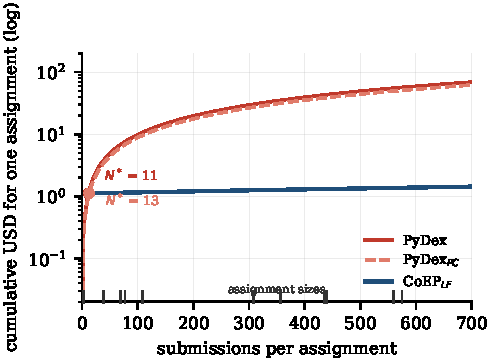
\includegraphics[width=\columnwidth]{figures/fig_cost.pdf}
\caption{Cumulative $C_{\mathrm{tot}}$ for one assignment against its
enrollment, solid for claude-sonnet-5 and dotted for gpt-5.4-mini. Dots mark
where \textsc{CoEP}\textsubscript{LF} overtakes each baseline; ticks along the
axis are the eleven assignments' actual sizes, ten of which clear $N^{*}$.}
\label{fig:cost}
\end{figure}


Three findings follow. \textbf{(1) In dollars}, \textsc{CoEP}\textsubscript{LF} spends $C_{\mathrm{tot}} = \$13.58$ over the whole benchmark on claude-sonnet-5 and \$1.00 on gpt-5.4-mini, against PyDex's \$292.77 and \$28.42, \textbf{21.6 and 28.4 times} ours, a ratio that scales with the $K{=}10$ candidates PyDex draws per submission and would be near 2$\times$ at $K{=}1$; prompt caching leaves PyDex\textsubscript{PC} at \$263.05 and \$23.50, \textbf{still 19.4 and 23.5 times}, because it pays for a shared leading \emph{prefix} and the variable buggy program comes first, leaving about ten identical tokens. \textbf{(2) In break-even}, an assignment repays its build after $N^{*}=\textbf{11}$ submissions against PyDex and 13 against PyDex\textsubscript{PC}, on claude-sonnet-5, and after 7 and 8 on gpt-5.4-mini, where the build falls faster (17.8$\times$) than the price of a query (10.3$\times$) and break-even therefore arrives sooner. Ten of the eleven assignments are past either point, most by an order of magnitude. \textbf{(3) In turnaround}, $\mathrm{ATT}_{\mathrm{tot}}$ is 3.06\,s against 14.64\,s on claude-sonnet-5 but 3.22\,s against 2.14\,s on gpt-5.4-mini, the one measure a per-submission arm can win, since a small model returns one completion faster than our search enumerates and re-executes candidates. PyDex\textsubscript{PC} re-prices queries rather than re-issuing them, so its turnaround is PyDex's exactly. What we pay for the first two is 22 minutes of build per assignment on claude-sonnet-5 (5.9--40.0), once and offline. Below $N^{*}$ a per-query repairer is the right tool; above it, and since every arm runs at the cheapest tier where caching functions, the measured gaps are a \emph{floor}.


\begin{table*}[t]
\centering\small\setlength{\tabcolsep}{3pt}
% BEGIN GENERATED tab_effect -- rewritten by `run.py tables`; do not edit
\begin{tabular}{crlc rrrrr c rrrrr}
\toprule
& & & & \multicolumn{5}{c}{\textbf{RR} (\%)} & & \multicolumn{5}{c}{\textbf{RPS}} \\
\cmidrule(lr){5-9}\cmidrule(lr){11-15}
& ID & Assignment & Rating & Refactory & PyDex & \textsc{CoEP}\textsubscript{fw} & \textsc{CoEP}\textsubscript{L} & \textsc{CoEP}\textsubscript{LF} & & Refactory & PyDex & \textsc{CoEP}\textsubscript{fw} & \textsc{CoEP}\textsubscript{L} & \textsc{CoEP}\textsubscript{LF} \\
\midrule
\multirow{5}{*}{\rotatebox[origin=c]{90}{\emph{Refactory}}} & R1 & Sequential search & -- & 99.0 & 99.7 & 100.0 & 100.0 & 100.0 & & 0.390 & 0.428 & 0.243 & 0.225 & 0.222 \\
 & R2 & Unique dates/months & -- & 78.2 & 97.8 & 91.3 & 93.8 & 97.9 & & 0.560 & 0.428 & 0.428 & 0.398 & 0.394 \\
 & R3 & Duplicate elimination & -- & 97.4 & 99.8 & 100.0 & 100.0 & 100.0 & & 0.340 & 0.423 & 0.284 & 0.280 & 0.280 \\
 & R4 & Sorting tuples & -- & 88.2 & 99.3 & 100.0 & 100.0 & 100.0 & & 0.310 & 0.535 & 0.388 & 0.386 & 0.291 \\
 & R5 & Top-$k$ elements & -- & 88.0 & 95.4 & 100.0 & 100.0 & 100.0 & & 0.320 & 0.244 & 0.196 & 0.193 & 0.191 \\
\midrule
\multirow{6}{*}{\rotatebox[origin=c]{90}{\emph{Codeforces}}} & C1 & Nearly Lucky Number & 800 & 85.2 & 99.9 & 100.0 & 100.0 & 100.0 & & 0.588 & 0.685 & 0.616 & 0.584 & 0.494 \\
 & C2 & cAPS lOCK & 1000 & 81.4 & 97.9 & 100.0 & 100.0 & 100.0 & & 0.724 & 1.167 & 0.841 & 0.762 & 0.648 \\
 & C3 & Planning Expedition & 1200 & 47.8 & 100.0 & 98.6 & 98.6 & 100.0 & & 0.847 & 0.705 & 0.640 & 0.638 & 0.585 \\
 & C4 & Measuring Lengths & 1400 & 92.1 & 100.0 & 100.0 & 100.0 & 100.0 & & 0.605 & 0.643 & 0.531 & 0.571 & 0.525 \\
 & C5 & Jumping Jack & 1600 & 40.3 & 100.0 & 100.0 & 100.0 & 100.0 & & 0.878 & 0.914 & 0.950 & 0.914 & 0.826 \\
 & C6 & Digital Root & 2000 & 100.0 & 100.0 & 100.0 & 100.0 & 100.0 & & 2.248 & 1.975 & 1.777 & 1.652 & 1.652 \\
\midrule
& \multicolumn{3}{l}{\textbf{Overall}} & \textbf{85.9} & \textbf{98.9} & \textbf{98.7} & \textbf{99.1} & \textbf{99.7} & & \textbf{0.500} & \textbf{0.634} & \textbf{0.492} & \textbf{0.463} & \textbf{0.410} \\
\bottomrule
\end{tabular}
% END GENERATED tab_effect
\caption{Overall repair effectiveness on 11 assignments, with the two builders
pooled. \textbf{RR} is the repair rate and \textbf{RPS} the relative patch size.
\textsc{CoEP}\textsubscript{fw} is the framework alone, the substrate with the
builder's rules removed, and uses no model at any point. Refactory's CS1 rows
are its published figures; its Codeforces rows are our run of the released
tool.}
\label{tab:effect}
\end{table*}

\subsubsection{RQ2: Repair Effectiveness.}


A repairer is judged on two things: how many submissions it fixes, and how much of the student's program it disturbs while fixing them. This question answers where a tool synthesized once per assignment stands on both, and how that varies across assignments. Table~\ref{tab:effect} reports per-assignment RR and RPS with the two builders pooled; RPS is averaged over what each arm repairs, so a low RPS beside a low repair rate means an easier subset rather than a better patch.


Three findings follow. \textbf{(1) Against the symbolic baseline}, the local tool alone repairs \textbf{99.1\%} at mean RPS \textbf{0.463} where Refactory repairs 85.9\% at 0.500, and its repair rate is at least Refactory's on every one of the eleven assignments. On Refactory's own corpus the same holds, 98.5\% against its published 90.8\% at 0.306 against 0.397. That comparison crosses instruments: 0.397 is the authors' figure, and measuring their tool the way we measure everyone gives 0.365, so the gap is 16\% rather than 23\%. Either way it costs no marginal LLM spend. \textbf{(2) Against per-submission LLM repair}, coverage is level: \textsc{CoEP}\textsubscript{L} reaches 99.1\% and PyDex 98.9\%, and adding the escalation tail takes \textsc{CoEP}\textsubscript{LF} to \textbf{99.7\%}, at 100\% on ten of the eleven assignments. What separates the arms is patch size, \textbf{0.463} against \textbf{0.634} and 0.410 for \textsc{CoEP}\textsubscript{LF}, 27\% and 35\% smaller, on ten and on all eleven assignments respectively. \textbf{(3) The per-assignment rows} show what a corpus mean hides, and what predicts it. Refactory's rate swings from 40.3\% to 100\% while no arm that consults a model drops below 93.8\%: grouped into bands, Refactory falls 90.8\% on CS1 to 83.1\% on Codeforces 800--1000 to \textbf{54.5\%} on 1200--2000, while \textsc{CoEP}\textsubscript{LF} holds 99.5/100.0/100.0. Thin pools alone do not explain that collapse, since C5 and C6 give every arm only two correct programs to work from and \textsc{CoEP}\textsubscript{fw}, which keeps the transplant and drops the builder's rules, repairs both at 100\%. What separates them is the granularity of reuse: Refactory adopts divergent blocks, so a pool that solves the problem another way leaves nothing adoptable, while we adopt line-hunks after renaming the reference program's variables to the student's, which stays applicable when the strategies differ. A low RPS is not always a virtue either: Refactory's 0.679 on Codeforces looks competitive against \textsc{CoEP}\textsubscript{LF}'s 0.597, but it is averaged over the 78.6\% it accepts, where \textsc{CoEP}\textsubscript{LF} repairs 100\%. Pooling the two builders hides nothing, finally: separately they reach 99.66\% at 0.404 RPS and 99.73\% at 0.417, three per cent apart in patch size for an eighteen-fold difference in build price. Overall, the synthesized tool beats the symbolic one on both coverage and patch size, matches per-submission LLM repair on coverage while disturbing a third less of the student's program, and does so on whichever builder writes it.


\begin{table}[t]
\centering\small\setlength{\tabcolsep}{3pt}
% BEGIN GENERATED tab_pool -- rewritten by `run.py tables`; do not edit
% END GENERATED tab_pool
\caption{Repair rate and patch size as the transplant's reference pool is
restricted to $k$ correct programs, over 146 submissions no builder was shown,
with brackets the range over three draws of each pool.}
\label{tab:pool}
\end{table}

\subsubsection{RQ3: Ablation Study.}


The previous two questions treated the tool as one object. This one opens it and asks what the model-authored rules add over the symbolic substrate beneath them. That substrate is \textsc{CoEP}\textsubscript{fw}: the identical tool with the builder's rules removed and the always-on rules and the transplant left in place, which uses no model at any point and is therefore the same artifact under either builder. It is a first-class arm in Table~\ref{tab:effect}, and Figure~\ref{fig:source} gives the decomposition the ablation acts on.


Three findings follow. \textbf{(1) The reach comes from the symbolic substrate.} \textsc{CoEP}\textsubscript{fw}, which never calls a model, repairs \textbf{98.69\%} at mean RPS \textbf{0.492}: far above Refactory's 85.93\%, and level on coverage with PyDex's 98.94\% at a smaller patch than its 0.634. We report this rather than bury it, because it is an unfavourable result for per-submission LLM repair and not for the reformulation. If 2{,}970 calls and \$292.77 buy a quarter of a point and a larger patch over a substrate that costs no model spend at all, that spending is the thing we are objecting to. \textbf{(2) The authored layer buys the last stretch above it.} Adding it takes the repair rate to 99.06\% and the mean patch to 0.463, and that 6\% patch reduction is diluted across the 75\% the transplant handles either way. On the \textbf{1{,}447} arm--submission pairs where a rule fires, 992 distinct programs, the rule's patch is RPS \textbf{0.100} against the substrate's \textbf{0.213} on the same programs, \textbf{2.1 times} larger without it, and on 13 of them the substrate produces no repair at all, though the fallback and PyDex both do. Labelling thins with it: repairs carrying a builder-written name fall from 17.8\% of all repairs to none, and only the always-on rules' names remain, over 10.1\%. We claim legibility for those names, not correctness: nothing here validates that a rule's name is the misconception a tutor would assign. \textbf{(3) The substrate's reach is borrowed from the pool.} Table~\ref{tab:pool} holds each tool fixed and varies only how many correct programs the transplant may draw on, over submissions no builder was shown, from ten assignments, with the claude-sonnet-5 tool. Down to one correct program coverage barely moves, half a point at most and inside the spread across draws, while the patch gap widens from 4\% to 12\%. Take the pool away entirely and the substrate has nothing to transplant from: it repairs \textbf{8.9\%} where the same tool with its rules repairs \textbf{29.5\%}. The rule layer is insurance against a thin pool, and a benchmark whose assignments each arrive with hundreds of correct submissions is precisely where that insurance looks worthless.  Whether \$1.11 per assignment is worth that is a departmental question, and a course sitting on a deep pool may reasonably decline. Our claim is not that the LLM produces the performance but that this is where LLM effort belongs.

\begin{figure}[h]
\centering
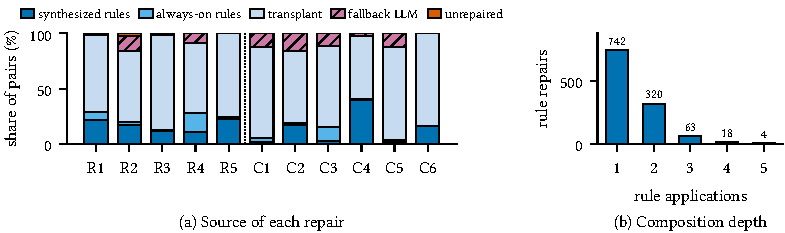
\includegraphics[width=\columnwidth]{figures/fig_source.pdf}
\caption{Decomposition of the ablation.}
\label{fig:source}
\end{figure}



\textbf{The rules sort by generality, and generality predicts reach.} \texttt{add\_missing\_call\_parens} names a Python trap that belongs to no assignment and is the only one of 128 to fire on two; \texttt{slice\_case\_check\_to\_equality} names C2's misconception and repairs 108 of its submissions; \texttt{carry\_fix\_two\_value\_print} is tied to C4's problem statement and repairs 28 of its 38 alone. That the layer is assignment-specific is a consequence of level, not a defect.

\subsubsection{RQ4: Self-Learning.}



The frozen tool leaves a record of what it could not repair. When the fallback then repairs one of those misses, the model generalizes that fix into a named rule, and the rule is kept only if the augmented tool repairs the miss on its own. This question answers whether such a rule holds outside the submission it was induced from. Absorption writes to a staging copy the evaluated pass never consults and the augmented tool is frozen before this arm runs, so the comparison is order-independent: the same submissions, the same acceptance rule, two rule sets. Of the 56 the frozen tool fails on, the fallback reaches 38 and the rules distilled from those reach 21 with no model at all; the supplement plots it.


Two findings follow. \textbf{(1) The material is scarce and the bar is high.} \textsc{CoEP}\textsubscript{L} fails on 56 of 5{,}940 submissions, the fallback repairs 38 of those, and those 38 attempts leave \textbf{8} rules, since a rule survives only if the augmented tool then repairs the miss on its own. That is not a failure of the mechanism but what a 99.06\% local repair rate means. \textbf{(2) The rules that survive generalize past the submissions that induced them.} All eight went on to repair, recovering \textbf{21} submissions between them, and since eight submissions induced them, \textbf{13} of those 21 are programs the rules had never seen. One submission regressed, so the net is 20, and the induction cost \$0.76 priced to the artifact. The cheaper builder gains more, on the same 27 abstentions on R2, which says the gain depends on how general a rule the model writes from one fix rather than on how much material it is given. Overall, self-learning fires only where the tool failed and such places are rare, but where it fires the rules carry past their own examples, for under a dollar per assignment.

\section{Conclusion}


We reformulate program repair for programming assignments so that the model writes the repair \emph{tool} rather than the patch, once per assignment, after which the frozen tool repairs submissions with no model at all. On 2{,}970 real student submissions it beats a reference-guided repairer on coverage and patch size and matches per-submission LLM repair at 21.6 times lower cost, repaying its build within 11 submissions. An ablation locates what the model buys: on deep reference pools it is smaller patches and a named misconception, and the reach becomes the model's only when the pool is taken away.

\bibliography{references}

\clearpage
\end{document}
